\section{Introduction}\label{section:introduction}

\emph{Starcraft: Brood Wars} is a Real Time Strategy (RTS) computer
game that has in recent years captured the attention of researchers on
game-playing artificial intelligence. Starcraft is a complex game,
including the fact that incomplete information is available for each
player, and that its actions are stochastic. Therefore it is a hard
and interesting challenge for Artificial Intelligence. Also it can be
approached from several levels, such as Strategic Planning, Execution
of tactical maneuvers, Estimation of hidden information, etc.

In this work, we focus on the problem of ``micro'' in
Starcraft. Micro, short for micromanagement, is the problem of
directly controlling a small number of units directly in an engagement
with units from an opponent player. The tasks required in micro
include moving damaged units out of the fire range from the enemy,
spreading the units to maximize the fire arc, and using an unit's
special abilities at the right time. Also, the decisions for each of
these tasks will differ according to the units controlled by the
player and the opponent.

Learning approaches for micro in Starcraft and other similar games has
been studied by many groups recently. For example, \citet{Shantia11ConnectionistSC}
created a micro controller focused
around a neural network that evaluate Q-values to be used by Sarsa;
\citet{Wender12ReinforcementMicroSC} explored Q-learning and Sarsa;
\citet{Zhen13NeuroEvoSC} compare NEAT and rtNEAT; and \citet{Liu14EffectiveMicro}
influence maps and potential fields.  Although each of these works uses a different
algorithm to generate the micro controller, one thing that they all
have in common is that they mostly measure success as the win rate,
i.e. the total number of combats won (although \citet{Liu14EffectiveMicro} does include
some measure of unit loss and survivors in their evaluation).

\begin{figure}
  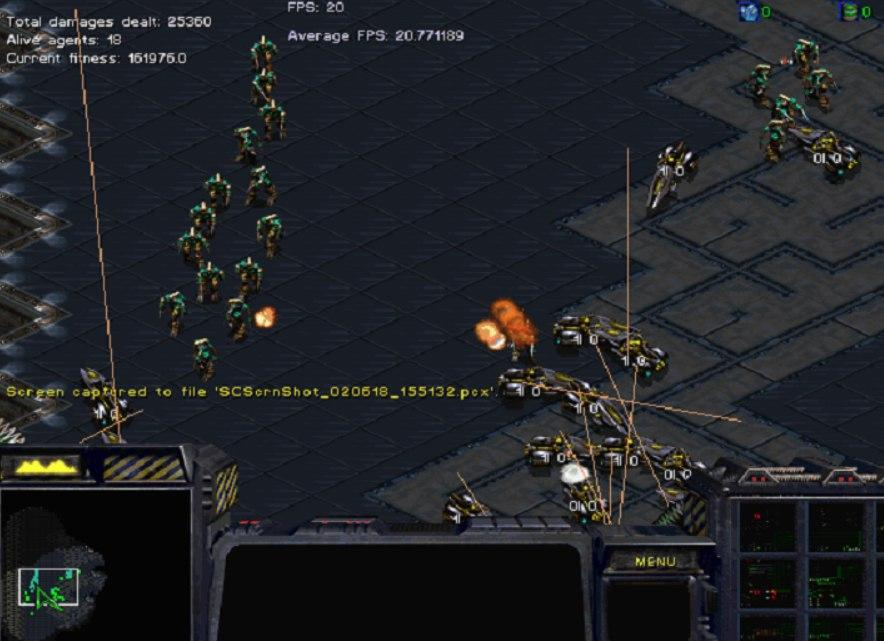
\includegraphics[width=.45\textwidth]{figures/vultures_vs_zealots_combat}
  \caption{Our AI controller leading vultures (right) against zealots
    (left). Our goal is to win small scale combats like this while
    reducing the number of lost units}
    \label{fig:combat-example}
\end{figure}

In this work we want to explore how to evolve a micro controller that
is able to not only achieve a high win rate, but also do so with as
few losses as possible. In an actual game, it is important for a player
to preserve their own forces, so that they can reallocate the remaining
forces to future battle, and compound their advantage through the match.

To achieve this, we propose an evaluation function that takes into
account the damages taken and the number of surviving units at the end
of a match, and compare four different NEAT implementations using this
utility function, as well as Novelty Search. We analyze the results of
four matchups (Marines vs Marines, Marines vs Zerg, Vultures vs
Vultures and Vultures vs Zealots). Quantitatively, none of the
implemented variants showed a strong difference from current
results. But a qualitative analysis indicate directions in the way
behaviours emerged.
